\documentclass[journal]{IEEEtran}

% Configure page layout and margins
\usepackage[a5paper, margin=10mm, onecolumn]{geometry}

% Essential packages for mathematics, symbols, and fonts
\usepackage{amsmath, amssymb, amsfonts, amsthm}
\usepackage{mathtools}
\usepackage{graphicx}
\usepackage{algorithmic}
\usepackage{listings}
\usepackage{xcolor}
\usepackage{multirow}
\usepackage{longtable}
\usepackage{gensymb}
\usepackage{tikz}
\usepackage{comment}
\usepackage[breaklinks=true]{hyperref}
\usepackage{txfonts}

% Bibliography style
\bibliographystyle{IEEEtran}

% Disable Gnumeric table input for now
\def\inputGnumericTable{}

% Begin document
\begin{document}

% Title and author information
\title{9.1.9}
\author{EE24BTECH11008 - Aslin Garvasis}
\maketitle

% Problem description
\textbf{Problem Statement:}\\
Solve the following second-order nonlinear differential equation:
\begin{equation}
y'' + y'^2 + 2y = 0
\end{equation}

% Solution approach
\textbf{Solution Approach:}\\
Finding an exact analytical solution for this nonlinear differential equation is challenging. Hence, we will use the numerical Euler method to obtain an approximate solution.

To apply Euler’s method, we first need to transform the second-order equation into a system of first-order equations.

Let:
\[
u = y' \quad \text{(First derivative of \( y \))}
\]
Thus, the second derivative becomes:
\[
u' = y''
\]

Substituting \( y' = u \) into the original equation gives:
\begin{equation}
u' + u^2 + 2y = 0
\end{equation}

This results in the following system of first-order differential equations:
\begin{align}
\frac{dy}{dx} &= u \\
\frac{du}{dx} &= -u^2 - 2y
\end{align}

This system can now be solved using Euler's method.

% Euler's method
\textbf{Euler’s Method:}\\
Euler's method approximates the solution of a system of first-order differential equations by updating the solution iteratively. The update rules are given by:
\begin{align}
y_{n+1} &= y_n + h \cdot u_n \\
u_{n+1} &= u_n + h \cdot (u'_n) \\
x_{n+1} &= x_n + h
\end{align}

Where:
- \( y_n \) and \( u_n \) are the values of \( y \) and \( u \) at the \( n \)-th step.
- \( h \) is the step size that controls the accuracy of the method.
- \( y_{n+1} \) and \( u_{n+1} \) are the updated values at the next step.

% Initial conditions
The initial conditions are:
\[
x_0 = 0.0, \quad y_0 = 0.1, \quad u_0 = -0.1, \quad h = 0.001
\]

The numerical solution was computed using these initial values, and the corresponding plot is shown below.

% Plot inclusion
\begin{figure}[h!]
    \centering
    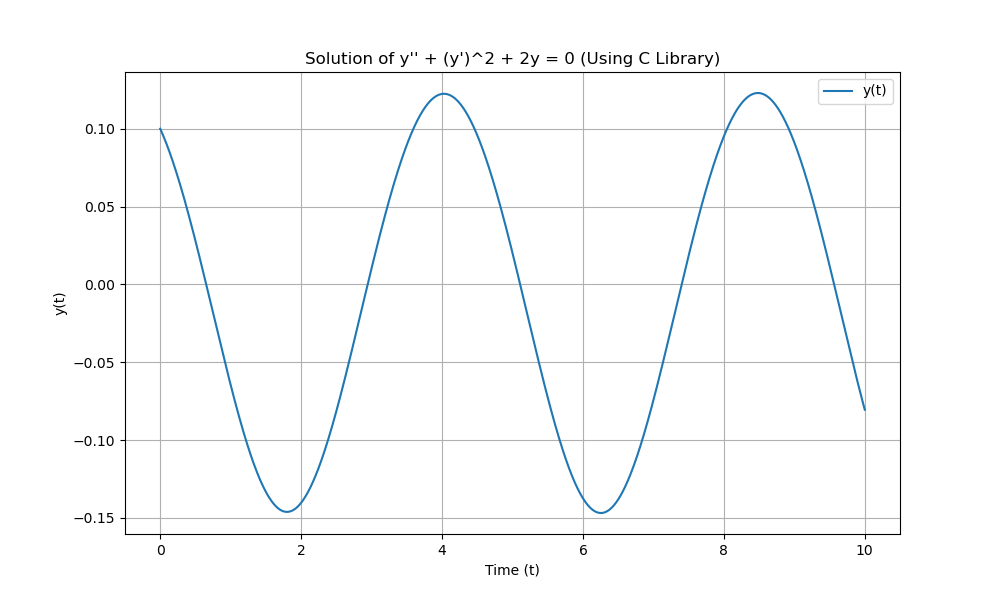
\includegraphics[width=\columnwidth]{figs/Fig 9.1.9.png}
    \caption{Numerical solution of the differential equation \( y'' + y'^2 + 2y = 0 \) using Euler's method.}
    \label{fig:solution_plot}
\end{figure}

\end{document}

